\chapter{Calculating Ground States with MPS}
For large systems exact diagonalization of the Hamiltonian is impossible, whereby one must resort to variational methods in order to find ground states. This involves finding the MPS, $\ket{\psi}$, which minimizes
\begin{equation}
	E = \frac{\bra{\psi} \hat{H} \ket{\psi}}{\braket{\psi | \psi}} \; .
\end{equation}
The most efficient way to do this, is to express the Hamiltonian as an MPO as described in eq. \eqref{eq:MPOrep}, whereby it easily can be applied to an MPS. While this may seem difficult at first, it can actually be done without any lengthy calculations. An example is given in Appendix \ref{chap:buildMPO}, where the Bose-Hubbard Hamiltonian is formulated as tensors.

\section{Efficient Application of a Hamiltonian to an MPS}
In section \ref{sec:MPO} it was explained how to apply an MPO to an MPS, and it was shown how to efficiently evaluate local operators. However, since $\hat{H} \ket{\psi}$ must be evaluated many times during variational methods, one must find even more efficient way of applying the operator.\\
Consider an MPS in a mixed-canonical form
\begin{align}
	\ket{\psi} &= \sum_{\boldsymbol{j}} A^{j_1} \ldots A^{j_{n-1}} \Psi^{j_n} B^{j_{n+1}} \ldots B^{j_{N}} \ket{\boldsymbol{j}} \nonumber \\
	&= \sum_{\alpha_{n-1} , \alpha_{n}} \ket{\alpha_{n-1}}_A \Psi_{\alpha_{n-1} , \alpha_{n}}^{j_n}  \ket{\alpha_{n}}_B \; ,
	\label{eq:MPSmixedsingle}
\end{align}
where $\Psi^{j_n}$ is the central site, and $\ket{\alpha_{n-1}}_A$ and $\ket{\alpha_{n}}_B$ are block states introduced in eq. \eqref{eq:mixedA} and \eqref{eq:mixedB} respectively.
Huge reductions in computational cost of the variational search can be found by re-using as many calculations as possible. In the basis $\{ \ket{\alpha_{n-1} } \; , \; \ket{ j_n } \; , \; \ket{\alpha_{n} } \}$ the individual matrix elements of the Hamiltonian can be expressed as
\begin{equation*}
	\bra{\alpha_{n-1} j_n \alpha_{n}} \hat{H} \ket{\alpha_{n-1} ' j_n ' \alpha_{n} '} = \sum_{\boldsymbol{j} , \boldsymbol{j'}}  W^{j_1 , j_1 '} \ldots W^{j_N , j_N '}  \braket{\alpha_{n-1} j_n \alpha_{n} | \boldsymbol{j}} \braket{\boldsymbol{j'} | \alpha_{n-1} ' j_n ' \alpha_{n} '} \; . 
\end{equation*}
Since the basis of local states $\{ \ket{\boldsymbol{j}} \}$ shares a state with the basis $\{ \ket{\alpha_{n-1} } \; , \; \ket{ j_n } \; , \; \ket{\alpha_{n} } \}$, the above expression can be re-written using $\sum_{\boldsymbol{j}} \braket{j_n | \boldsymbol{j}} = \sum_{\boldsymbol{j *}} \ket{ \boldsymbol{j *}}$, where "$\boldsymbol{*}$" means "excluding $j_n$". Thus,
\begin{align}
&	\bra{\alpha_{n-1} j_n \alpha_{n}} \hat{H} \ket{\alpha_{n-1} ' j_n ' \alpha_{n} '} = \nonumber \\
 &= \sum_{\boldsymbol{j *} , \boldsymbol{j' * }}  W^{j_1 , j_1 '} \ldots W^{j_n , j_n '} \ldots W^{j_N , j_N '} \nonumber \\
	& \qquad \times \braket{\alpha_{n-1} | j_1 \ldots j_{n-1}} \braket{\alpha_{n} | j_{n+1} \ldots j_{N}} \braket{j_1 ' \ldots j_{n-1} ' | \alpha_{n-1} '} \braket{j_{n+1} ' \ldots j_{N} ' | \alpha_{n} '} \nonumber \\
	&= \sum_{\boldsymbol{j *} , \boldsymbol{j' * }}  W^{j_1 , j_1 '} \ldots W^{j_n , j_n '} \ldots W^{j_N , j_N '} \nonumber \\
	& \qquad \times \left( A^{j_1} \ldots A^{j_{n-1}} \right)_{1 , \alpha_{n-1}}^{*} \left( B^{j_{n+1}} \ldots B^{j_{N}} \right)_{ \alpha_{n} , 1}^{*} \left( A^{j_1 '} \ldots A^{j_{n-1} '} \right)_{1 , \alpha_{n-1} '} \left( B^{j_{n+1} '} \ldots B^{j_{N} '} \right)_{ \alpha_{n} ' , 1} \nonumber \\
	&= \sum_{\alpha_n , \beta_n , \alpha_n '}
	\left( \sum_{j_1 , j_1 '} A_{1 , \alpha_1}^{j_1 *} W_{1, \beta_1}^{j_1 , j_1 '} A_{1 , \alpha_1 '}^{j_1 '} \right)
	\left( \sum_{j_2 , j_2 '} A_{\alpha_1 , \alpha_2}^{j_2 *} W_{\beta_1, \beta_2}^{j_2 , j_2 '} A_{\alpha_1 ' , \alpha_2 '}^{j_2 '} \right)
	\ldots W_{\beta_{n_1}, \beta_n}^{j_n , j_n '} \nonumber \\
	& \qquad \times \left( \sum_{j_{n+1} , j_{n+1} '} B_{\alpha_n , \alpha_{n+1}}^{j_{n+1} *} W_{\beta_n, \beta_{n+1}}^{j_{n+1} , j_{n+1} '} B_{\alpha_n ', \alpha_{n+1} '}^{j_{n+1} '} \right)
	\left( \sum_{j_{N} , j_{N} '} B_{\alpha_{N-1} , 1}^{j_{N} *} W_{\beta_{N-1}, 1}^{j_{N} , j_{N} '} B_{\alpha_{N-1}' , 1 }^{j_{N} '} \right)  \; .
\end{align}  
While this expression may seem terrible complicated due to all the indices, it is actually rather easy to understand. First, the matrix element is written excluding the local basis state $\ket{j_n}$. Next, the Hamilton MPO is projected into the block states of A, $\ket{\alpha_{n-1}}_A$, and B, $\ket{\alpha_{n}}_B$. Finally, the matrices are grouped according to their expansion in the local basis. Working with the above expression appears cumbersome, but it is merely a decoupling of the system into three distinct parts, which can be seen in figure \ref{fig:singleElemHamil}.
\begin{figure}[h!]
	\centering
	\begin{tikzpicture}[inner sep=1mm]
    \foreach \i in {1,...,4} {
        \node[tensor] (tt\i) at (2* \i -1, 0) {};
        \node[operator] (o\i) at (2* \i -1, -1.5) {};
        \node[tensor] (tb\i) at (2* \i -1, -3) {};
        
        
        \draw[-] (tt\i) -- (o\i);
        \draw[-] (o\i) -- (tb\i);
    };
    \foreach \i in {6,...,7} {
        \node[tensor] (tt\i) at (2* \i -1, 0) {};
        \node[operator] (o\i) at (2* \i -1, -1.5) {};
        \node[tensor] (tb\i) at (2* \i -1, -3) {};
        
        
        \draw[-] (tt\i) -- (o\i);
        \draw[-] (o\i) -- (tb\i);
    };
        \foreach \i in {1,...,3} {
        \pgfmathtruncatemacro{\iplusone}{\i + 1};
        \draw[-] (tt\i) -- (tt\iplusone);
        \draw[-] (tb\i) -- (tb\iplusone);
        \draw[-] (o\i) -- (o\iplusone);
    };
    \draw[-] (tt6) -- (tt7);
    \draw[-] (tb6) -- (tb7);
    \draw[-] (o6) -- (o7);
    
    
       
	\node[operator] (o5) at (2* 5 -1, -1.5) {};    
    
    \node (a1) at (8,0.5) {$\alpha_{n-1}$};
    \node (a2) at (10,0.5) {$\alpha_{n}$};
    \node (a1p) at (8,-3.5) {$\alpha_{n-1} '$};
    \node (a2p) at (10,-3.5) {$\alpha_{n} '$};
    \node (j) at (9,-0.5) {$j_n$};
    \node (jp) at (9,-2.5) {$j_n '$};
    
    \node (a1d) at (8,0) {};
    \node (a2d) at (10,0) {};
    \node (a1pd) at (8,-3) {};
    \node (a2pd) at (10,-3) {};
    
    \draw[-] (tt4) -- (a1d);
    \draw[-] (tt6) -- (a2d);
    \draw[-] (tb4) -- (a1pd);
    \draw[-] (tb6) -- (a2pd);
    \draw[-] (o5) -- (j);
    \draw[-] (o5) -- (jp);
    \draw[-] (o5) -- (o4);
    \draw[-] (o5) -- (o6);
    
    \node (d1) at (8,-0.75) {};
    \node (d2) at (8,-2.25) {};
   	\draw[dashed] (d1) -- (d2);
   	\node (d3) at (10,-0.75) {};
    \node (d4) at (10,-2.25) {};
   	\draw[dashed] (d3) -- (d4);
   	
   	
   	\node (L) at (4,-4.5) {L};
   	\node (W) at (9,-4.5) {W};
   	\node (R) at (12,-4.5) {R};
\end{tikzpicture}
	\caption{\textit{Representation of the matrix element $\bra{\alpha_{n-1} j_n \alpha_{n}} \hat{H} \ket{\alpha_{n-1} ' j_n ' \alpha_{n} '}$ as an tensor network. Expressing the matrix element in this form decouples the network in three parts: The matrices of the MPO, $W^{[n]}$, connecting the physical sites of the matrix element, and contracted parts L and R consisting of the rest of the MPO and the left- and right-normalised part of the MPS respectively.}}
	\label{fig:singleElemHamil}
\end{figure}
Since both the left and right side of the network is connected, one can contract these parts into two separate tensors $L$ and $R$ called "environments":
\begin{align}
	L_{\alpha_{n-1}, \beta_{n-1} , \alpha_{n-1} '} &= \sum_{ \substack{ \{ \alpha_i \beta_i \alpha_i ' \} \\ i < n-1}} \left( \sum_{j_1 , j_1 '} A_{1 , \alpha_1}^{j_1 *} W_{1, \beta_1}^{j_1 , j_1 '} A_{1 , \alpha_1 '}^{j_1 '} \right) \ldots \left( \sum_{j_{n-1} , j_{n-1} '} A_{\alpha_{n-2} , \alpha_{n-1}}^{j_{n-1} *} W_{\beta_{n-2}, \beta_{n-1}}^{j_{n-1} , j_{n-1} '} A_{\alpha_{n-2} ' , \alpha_{n-1} '}^{j_{n-1} '} \right) \label{eq:Ltensor} \\
	R_{\alpha_{n} ,\beta_{n} , \alpha_{n} '} &= \sum_{ \substack{ \{ \alpha_i \beta_i \alpha_i ' \} \\ i > n}} \left( \sum_{j_{n+1} , j_{n+1} '} B_{\alpha_n , \alpha_{n+1}}^{j_{n+1} *} W_{\beta_n, \beta_{n+1}}^{j_{n+1} , j_{n+1} '} B_{\alpha_n ', \alpha_{n+1} '}^{j_{n+1} '} \right) \left( \sum_{j_{N} , j_{N} '} B_{\alpha_{N-1} , 1}^{j_{N} *} W_{\beta_{N-1}, 1}^{j_{N} , j_{N} '} B_{\alpha_{N-1}' , 1 }^{j_{N} '} \right) \label{eq:Rtensor}
\end{align}
From these contractions, the obvious tripartite structure of the Hamiltonian matrix element, as seen in figure \ref{fig:singleElemHamil}, can be written in a compact way
\begin{equation}
	\bra{\alpha_{n-1} j_n \alpha_{n}} \hat{H} \ket{\alpha_{n-1} ' j_n ' \alpha_{n} '} = \sum_{\beta_{n-1} , \beta_{n}} L_{\alpha_{n-1}, \beta_{n-1} , \alpha_{n-1} '} \; W_{\beta_{n_1}, \beta_n}^{j_n , j_n '} \; R_{\alpha_{n} ,\beta_{n} , \alpha_{n} '} \; .
\end{equation}
Finally, applying this parametrization of the Hamiltonian to the MPS of eq. \eqref{eq:MPSmixedsingle} yields \cite{schollwock}
\begin{equation}
	\hat{H} \ket{\psi} = \sum_{\beta_{n-1} , \beta_{n}} \sum_{\alpha_{n-1}' , j_n ', \alpha_{n}'} L_{\alpha_{n-1}, \beta_{n-1} , \alpha_{n-1} '} \; W_{\beta_{n_1}, \beta_n}^{j_n , j_n '} \; R_{\alpha_{n} ,\beta_{n} , \alpha_{n} '} \; \Psi_{\alpha_{n-1} ' , \alpha_{n} '}^{j_n '} \ket{\alpha_{n-1}}_A \ket{j_n} \ket{\alpha_{n}}_B \; .
	\label{eq:HPsi}
\end{equation}
As mentioned earlier, evaluating $\hat{H} \ket{\psi}$ must be done many times during a variational search of the ground state, hence this operation must be executed as fast as possible. Examining eq. \eqref{eq:HPsi} one will notice, that while the boundaries of $L$ and $R$ will change depending on which site is being optimized, the bulk of the two tensors remain constant through a lot of the calculations. Instead of calculating $L$ and $R$ from eq. \eqref{eq:Ltensor} and \eqref{eq:Rtensor} for every evaluation of eq. \eqref{eq:HPsi}, one can iteratively build them, since they only change by one column of the network at a time. Thus, a large number of computations can be reused.\\
Consider the construction of the tensor $L^{[i]}$. This can be built iteratively from the left by contracting the previous left-tensor $L^{[i-1]}$ with the i'th column of the network consisting of $A^{[i]}$, $W^{[i]}$ and $A^{[i] \dag}$
\begin{equation}
	L_{\alpha_i , \beta_i , \alpha_i '}^{[i]} = \sum_{\substack{ j_i , j_i ' \\ \alpha_{i-1} , \beta_{i-1} , \alpha_{i-1} '}} W_{\beta_{i-1} , \beta_i}^{[i] j_i , j_i '} \left( A^{[i] j_i \dag} \right)_{\alpha_i , \alpha_{i-1}} L_{\alpha_{i-1} , \beta_{i-1} , \alpha_{i-1} '}^{[i-1]} A_{\alpha_{i-1} ' , \alpha_i '}^{[i] j_i '} \; .
\end{equation}
This iterative update of $L^{[i]}$ can be seen illustrated in figure \ref{fig:buildLTensor}. The square-bracket notation has been re-introduced to keep track of the tensors relation to the physical sites. In order to remain consistent with notation, the dummy scalars $L_{\alpha_0 , \beta_0 , \alpha_0 '}^{[0]}  = 1  = \alpha_0 , \beta_0 , \alpha_0 '$ has been introduced.\\
\begin{figure}[h!]
	\centering
	\begin{tikzpicture}[inner sep=1mm]
    \foreach \i in {1,...,3} {
        \node[tensor] (tt\i) at (\i, 0) {};
        \node[operator] (o\i) at (\i, -1.5) {};
        \node[tensor] (tb\i) at (\i, -3) {};  
        
        \draw[-] (tt\i) -- (o\i);
        \draw[-] (o\i) -- (tb\i);
    };
    \foreach \i in {1,...,2} {
        \pgfmathtruncatemacro{\iplusone}{\i + 1};
        \draw[-] (tt\i) -- (tt\iplusone);
        \draw[-] (tb\i) -- (tb\iplusone);
        \draw[-] (o\i) -- (o\iplusone);
    };
    \foreach \i in {9,...,12} {
        \node[tensor] (tt\i) at (\i, 0) {};
        \node[operator] (o\i) at (\i, -1.5) {};
        \node[tensor] (tb\i) at (\i, -3) {};  
        
        \draw[-] (tt\i) -- (o\i);
        \draw[-] (o\i) -- (tb\i);
    };
    \foreach \i in {9,...,11} {
        \pgfmathtruncatemacro{\iplusone}{\i + 1};
        \draw[-] (tt\i) -- (tt\iplusone);
        \draw[-] (tb\i) -- (tb\iplusone);
        \draw[-] (o\i) -- (o\iplusone);
    };
    
    \node[tensor] (tt4) at (5.4, 0) {};
    \node[operator] (o4) at (5.4, -1.5) {};
    \node[tensor] (tb4) at (5.4, -3) {};

	\draw[-] (tt4) -- (o4);
	\draw[-] (tb4) -- (o4);
    
    \node (at1) at (4.3, 0) {$\alpha_{i-1}$};
    \node (at2) at (6.4, 0) {$\alpha_{i}$};
    \node (ab1) at (4.3, -3) {$\alpha_{i-1} '$};
    \node (ab2) at (6.4, -3) {$\alpha_{i} '$};
    \node (b1) at (4.3, -1.5) {$\beta_{i-1}$};
    \node (b2) at (6.4, -1.5) {$\beta_{i}$};
    
    \draw[-] (tt3) -- (at1);
    \draw[-] (tb3) -- (ab1);
    \draw[-] (o3) -- (b1);
    \draw[-] (tt4) -- (at1);
    \draw[-] (tb4) -- (ab1);
    \draw[-] (o4) -- (b1);
    \draw[-] (tt4) -- (at2);
    \draw[-] (tb4) -- (ab2);
    \draw[-] (o4) -- (b2);
    
    
    \draw[->, line width=1mm] (6.9,-1.5) -- (8.4,-1.5);
    
    \node (at3) at (13, 0) {$\alpha_{i}$};
    \node (ab3) at (13, -3) {$\alpha_{i} '$};
    \node (b3) at (13, -1.5) {$\beta_{i}$};
    \draw[-] (tt12) -- (at3);
    \draw[-] (tb12) -- (ab3);
    \draw[-] (o12) -- (b3);
    
    \node (L1) at (2,-4) {$L^{[i-1]}$};
    \node (L2) at (10.5,-4) {$L^{[i]}$};

    
    \node (eq) at (14,-1.5) {$\equiv$};
    

    \node (dummy1) at (16,0) {$\alpha_{i}$};
 	\node (dummy2) at (16,-3) {$\alpha_{i} '$};
 	\node (dummy3) at (16,-1.5) {$\beta_{i}$};
	\node[tensor] (mat) at (15 , -1.5) {};    
    
    \draw[-] (dummy1.west) .. controls (15, 0) .. (mat.north);
    \draw[-] (dummy2.west) .. controls (15, -3) .. (mat.south);
	\draw[-] (mat) -- (dummy3);   
	
	
	\node (L3) at (15.5,-4) {$L^{[i]}$}; 
\end{tikzpicture}
	\caption{\textit{Iterative update from $L^{[i-1]}$ to $L^{[i]}$. This is done through a contraction of $L^{[i-1]}$ with $A^{[i]}$, $W^{[i]}$ and $A^{[i] \dag}$. The result is a tensor with three horizontal legs.}}
	\label{fig:buildLTensor}
\end{figure}
It is important to store every iteration of $L^{[i]}$, since $L$ will grow and shrink constantly throughout the variational search of the ground state, whereby every iteration of $L^{[i]}$ will be used multiple times.
The same applies when building the right environment, $R$. Here one starts from the right and moves left when iteratively contracting the tensor. By applying optimal bracketing, the computational cost of updating the environments scales as $\mathrm{O}(d D^3 D_W)$.
  

\section{Iterative Ground State Search and the DMRG Algorithm} \label{sec:DMRG}
In order to find the ground state of the system on can introduce a Lagrangian multiplier, $\lambda$, and extremize
\begin{equation}
	\bra{\psi} \hat{H} \ket{\psi} - \lambda \braket{\psi | \psi} \; ,
	\label{eq:lagrange}
\end{equation}
whereby the desired ground state, $\ket{\psi}$, and ground state energy, $\lambda^0$, will be reached.\\
Trying to optimize an entire MPS at once is a highly non-linear problem involving an extremely large number of variables. However, the problem can be linearised by only considering the variables of a single tensor (site) at a time, while keeping the rest of the MPS constant. By varying just a single tensor at a time, one will continuously find states lower in energy, until convergence is reached. However, this procedure is very prone to getting stuck in a local extrema. To circumvent this, one can consider two sites at a time and optimize with regards to a two-site tensor, created by momentarily merging the two sites \cite{WhiteDMRG}.\\
Consider the variation of the tensors $M^{[n]}$ and $M^{[n+1]}$. Expressing the minimization problem of eq. \eqref{eq:lagrange} in terms of the left and right environments (as done in eq. \eqref{eq:HPsi}) yields
\begin{align}
	\bra{\psi} \hat{H} \ket{\psi} &= \sum_{\substack{j_n , j_n ' \\ j_{n+1} , j_{n+1} '}} \sum_{\alpha_{n-1} ' , \alpha_n ', \alpha_{n+1} '} \sum_{\alpha_{n-1} , \alpha_n , \alpha_{n+1}} \sum_{\beta_{n-1} , \beta_n , \beta_{n+1}} L_{\alpha_{n-1}, \beta_{n-1} , \alpha_{n-1} '}^{[n-1]} \; W_{\beta_{n_1}, \beta_n}^{[n] j_n , j_n '} \; W_{\beta_{n}, \beta_{n+1}}^{[n+1] j_{n+1} , j_{n+1} '} \nonumber \\
	& \qquad \times R_{\alpha_{n+1} ,\beta_{n+1} , \alpha_{n+1} '}^{[n+2]} \; M_{\alpha_{n-1} , \alpha_{n}}^{[n] j_n } \; M_{\alpha_{n-1} ' , \alpha_{n} '}^{[n] j_n ' *} \; M_{\alpha_{n} , \alpha_{n+1}}^{[n+1] j_{n+1} } \; M_{\alpha_{n} ' , \alpha_{n+1} '}^{[n+1] j_{n+1} ' *}  \label{eq:twositeHamil}\\
	\braket{\psi | \psi} &= \sum_{j_n , j_{n+1} } \sum_{\substack{\alpha_{n-1} ' \\ \alpha_n ', \alpha_{n+1} '}} \sum_{\substack{\alpha_{n-1} , \alpha_n \\ \alpha_{n+1}}} \Psi_{\alpha_{n-1},\alpha_{n-1}'}^{A} \; M_{\alpha_{n-1} , \alpha_{n}}^{[n] j_n } \; M_{\alpha_{n-1} ' , \alpha_{n} '}^{[n] j_n ' *} \; M_{\alpha_{n} , \alpha_{n+1}}^{[n+1] j_{n+1} } \; M_{\alpha_{n} ' , \alpha_{n+1} '}^{[n+1] j_{n+1} ' *} \; \Psi_{\alpha_{n+1},\alpha_{n+1}'}^{B} \; , \label{eq:twositeOverlap}
\end{align}
where the Hamiltonian from eq. \eqref{eq:HPsi} has been re-ordered to accommodate examining two sites, $n$ and $n+1$, at a time, and 
\begin{align}
\Psi_{\alpha_{n-1},\alpha_{n-1}'}^{A} &= \sum_{j_1 , \ldots , j_{n-1}} \left( M^{j_{n-1} \dag} \ldots M^{j_{1} \dag} M^{j_1} \ldots M^{j_{n-1}} \right) _{\alpha_{n-1} , \alpha_{n-1} '} \label{eq:psiA} \\
\Psi_{\alpha_{n+1},\alpha_{n+1}'}^{B} &= \sum_{j_{n+2} , \ldots , j_{N}} \left( M^{j_{n+2} } \ldots M^{j_{N} } M^{j_N \dag} \ldots M^{j_{n+2} \dag} \right) _{\alpha_{n+1} ', \alpha_{n+1} } \; .
\end{align}
Further simplifications can be made for mixed-canonical forms, if sites $1$ through $n-1$ are left-normalized, and sites $n+2$ through $N$ are right-normalized, whereby
\begin{equation}
	\Psi_{\alpha_{n-1},\alpha_{n-1}'}^{A} = \delta_{\alpha_{n-1},\alpha_{n-1}'} \qquad , \qquad \Psi_{\alpha_{n+1},\alpha_{n+1}'}^{B} = \delta_{\alpha_{n+1},\alpha_{n+1}'} \; .
\end{equation}
Finding the extremum of eq. \eqref{eq:lagrange} with respect to $M_{\alpha_{n-1} ' , \alpha_{n} '}^{[n] j_n ' *} \; M_{\alpha_{n} ' , \alpha_{n+1} '}^{[n+1] j_{n+1} ' *}$ is done through the following sequence:

\subsection{Two-site update for iterative ground state search}
\begin{enumerate}
\item
\textbf{Merge:} Contract the two matrices $M^{[n]}$ and $M^{[n+1]}$ over the bond $\alpha_{n}$ creating a two-site tensor
\begin{equation}
\Theta_{\alpha_{n-1} , \alpha_{n+1}}^{j_n , j_{n+1}} = \sum_{\alpha_n} M_{\alpha_{n-1} , \alpha_{n}}^{[n] j_n } \;  M_{\alpha_{n} , \alpha_{n+1}}^{[n+1] j_{n+1} } 
\end{equation}

\item
\textbf{Solve eigenproblem:} This yields an eigenvalue problem, which can be seen by reshaping
\begin{align}
	H_{( \alpha_{n-1}  j_n  j_{n+1}, \alpha_{n+1}),(\alpha_{n-1}'  j_n '  j_{n+1}', \alpha_{n+1}')} &= \nonumber \\
	= \; \sum_{\substack{\beta_{n-1} , \beta_n \\ \beta_{n+1}}} L_{\alpha_{n-1}, \beta_{n-1} , \alpha_{n-1} '}^{[n-1]} & \; W_{\beta_{n_1}, \beta_n}^{[n] j_n , j_n '} \; W_{\beta_{n}, \beta_{n+1}}^{[n+1] j_{n+1} , j_{n+1} '}\;  R_{\alpha_{n+1} ,\beta_{n+1} , \alpha_{n+1} '}^{[n+2]} \\
	v_{ \alpha_{n-1} j_n j_{n+1} \alpha_{n+1}} &= \; \Theta_{\alpha_{n-1} , \alpha_{n+1}}^{j_n , j_{n+1}}
\end{align}
such that
\begin{equation}
	H v - \lambda v = 0 \; .
	\label{eq:eigprob}
\end{equation}
Solving this for the lowest eigenvalue $\lambda_0$ yields $v_{ \alpha_{n-1} j_n j_{n+1} \alpha_{n+1}}^0$, which can be reshaped back to the now optimized two-site tensor, $\tilde{\Theta}_{\alpha_{n-1} , \alpha_{n+1}}^{j_n , j_{n+1}}$.

\item
\textbf{Unmerge:} Reshape the updated $\tilde{\Theta}_{\alpha_{n-1} , \alpha_{n+1}}^{j_n , j_{n+1}}$ to a matrix and perform an SVD yielding
\begin{equation}
	\tilde{\Theta}_{(j_n \alpha_{n-1} ) ,(j_{n+1}  \alpha_{n+1} )} = \sum_{\alpha_n} U_{\alpha_{n-1} , \alpha_{n}}^{j_n} S_{\alpha_n , \alpha_n} (V^{\dag})_{\alpha_{n} , \alpha_{n+1}}^{j_{n+1}} \; .
\end{equation}
This causes the bond dimension to increase $D \rightarrow d D$, which must be truncated by keeping only the $D$ largest singular values of $S$. 

\item
\textbf{Update environments:} The last step depends on which direction, one is iterating trough the chain. Here, the left- and right-normalization of $U$ and $V^{\dag}$ is used to update the environments.\\
\textit{Going right}: Update the left environment
\begin{equation}
	\tilde{L}_{\alpha_{n}, \beta_{n} , \alpha_{n} '}^{[n]} = \sum_{\substack{ j_{n} , j_{n} ' \\ \alpha_{n-1} , \beta_{n-1} , \alpha_{n-1} '}} L_{\alpha_{n-1}, \beta_{n-1} , \alpha_{n-1} '}^{[n-1]} \; U_{\alpha_{n-1} , \alpha_{n}}^{j_n} \; W_{\beta_{n-1} , \beta_{n}}^{[n] j_n , j_n '} \; U_{\alpha_{n-1} ', \alpha_{n}'}^{j_n ' *} \; ,
\label{eq:updateLeft}
\end{equation}
and build the matrix of the right site
\begin{equation}
	\tilde{M}_{\alpha_{n} , \alpha_{n+1}}^{[n+1] j_{n+1} } = \sum_{\alpha_n}  S_{\alpha_n , \alpha_n} (V^{\dag})_{\alpha_{n} , \alpha_{n+1}}^{j_{n+1}} \; .
\end{equation}\\ 
\textit{Going left}: Update the right environment
\begin{equation}
	\tilde{R}_{\alpha_{n}, \beta_{n} , \alpha_{n} '}^{[n+1]} = \sum_{\substack{ j_{n+1} , j_{n+1} ' \\ \alpha_{n+1} , \beta_{n+1} , \alpha_{n+1} '}} R_{\alpha_{n+1}, \beta_{n+1} , \alpha_{n+1} '}^{[n+2]} \; \left( V^{\dag} \right)_{\alpha_{n} , \alpha_{n+1}}^{j_{n+1}} \; W_{\beta_{n} , \beta_{n+1}}^{[n+1] j_{n+1} , j_{n+1} '} \; \left( V^{\dag} \right)_{\alpha_{n} , \alpha_{n+1}}^{j_{n+1} *} \; ,
	\label{eq:updateRight}
\end{equation}
and build the matrix of the left site
\begin{equation}
	\tilde{M}_{\alpha_{n-1} , \alpha_{n}}^{[n] j_{n} } = \sum_{\alpha_n} U_{\alpha_{n-1} , \alpha_{n}}^{j_n} S_{\alpha_n , \alpha_n}  \; .
\end{equation} 
 
\end{enumerate}
This concludes the two-site update sequence, which is illustrated in figure \ref{fig:twoSiteUpdate}. After performing the sequence, one can move \textit{one site} to either left or right, depending on which direction, one is iterating.

\renewcommand{\thesubfigure}{\arabic{subfigure}}
\begin{figure}[h!]
	\centering
	\begin{subfigure}{\textwidth}
		\centering
		\caption{\textbf{Merge:}}
		\begin{tikzpicture}[inner sep=1mm]
	\def \imgcenter {5.25};
	\def \imgwidth {15};
	\node[minimum width=\imgwidth cm] (fake) at (\imgcenter ,0) {};


    \node[tensor] (M1) at (1 , 0) {};
    \node[tensor] (M2) at (2.5 , 0) {};
	\node[tensor, minimum width=2cm] (sig) at (9, 0) {};
	
	\node (j1) at (1 ,-1) {$j_n$};
	\node (j2) at (2.5 ,-1) {$j_{n+1}$};
	\node (a1) at (-0.2 ,0) {$\alpha_{n-1}$};
	\node (a2) at (3.7 ,0) {$\alpha_{n+1}$};    
    
	\draw[-] (M1) -- (j1);
	\draw[-] (M1) -- (a1);
	\draw[-] (M1) -- (M2);
	\draw[-] (M2) -- (j2);
	\draw[-] (M2) -- (a2);
	
	
	\node (node1) at (8.35, -1) {$j_n$};
	\node (node2) at (9.65, -1) {$j_{n+1}$};
	\node (as1) at (7 ,0) {$\alpha_{n-1}$};
	\node (as2) at (11 ,0) {$\alpha_{n+1}$};
	
	\draw[-] (node1) -- (node1 |-  sig.south);
	\draw[-] (node2) -- (node2 |-  sig.south);
	\draw[-] (sig) -- (as1);
	\draw[-] (sig) -- (as2);		
	
	\draw[->, line width=1mm] (4.5,0) -- (6,0);
	
	\node (Mlab1) at (1,0.8) {$M^{[n]}$};
	\node (Mlab2) at (2.5,0.8) {$M^{[n+1]}$};
	\node (Siglab) at (9,0.6) {$\Theta$};
	
	
\end{tikzpicture}
	\end{subfigure}\\[.8cm]
	
	\begin{subfigure}{\textwidth}
		\centering
		\caption{\textbf{Solve eigenprobem:}}
		\begin{tikzpicture}[inner sep=1mm]
	\def \imgcenter {5.8};
	\def \imgwidth {15};
	\node[minimum width=\imgwidth cm] (fake) at (\imgcenter ,0) {};	
	
	
	\node[tensor, minimum width=2.5cm] (theta) at (2, 0) {};
	\node[operator] (W1) at (1.1,-1.5) {};
	\node[operator] (W2) at (2.9,-1.5) {};	
	
	\node (dummy1) at (0.3,-3) {};
 	\node (dummy2) at (3.6,-3) {};
	\node[tensor] (L) at (-0.5 , -1.5) {};
	\node[tensor] (R) at (4.5 , -1.5) {};    
    
    \draw[-] (dummy1.west) .. controls (-0.5, -3) .. (L.south);
    \draw[-] (dummy2.east) .. controls (4.5, -3) .. (R.south);
    \draw[-] (theta.west) .. controls (-0.5, 0) .. (L.north);
    \draw[-] (theta.east) .. controls (4.5, 0) .. (R.north);
	
	\draw[-] (L) -- (W1);
	\draw[-] (W1) -- (W2);
	\draw[-] (W2) -- (R);
	\draw[-] (W1) -- (W1 |-  theta.south);
	\draw[-] (W2) -- (W2 |-  theta.south);
	
	\node (j1) at (1.1 , -2.5) {$j_{n}'$};
	\node (j2) at (2.9 , -2.5) {$j_{n+1}'$};
	\draw[-] (W1) -- (j1);
	\draw[-] (W2) -- (j2);
	
	\node (a1) at (0.5 , -3.3) {$\alpha_{n-1}'$};
	\node (a2) at (3.6 , -3.3) {$\alpha_{n+1}'$};
	\node (Llab) at (-1.2 , -1.5) {$L$};
	\node (Rlab) at (5 , -1.6) {$R$};	
	\node (Thetalab) at (2 , 0.6) {$\tilde{\Theta}$};
	\node (W1lab) at (0.6 , -0.9) {$W^{[n]}$};
	\node (W2lab) at (3.6 , -0.9) {$W^{[n+1]}$};
	
	
	\def \offsetx {7.5};
	\def \offsety {-1};
	\node[tensor, minimum width=2.5cm] (theta2) at (2+\offsetx, \offsety) {};
	\node (d1) at (1.1 +\offsetx, -1+ \offsety) {};
	\node (d2) at (2.9 +\offsetx, -1 + \offsety) {};
	\node (d3) at (2+\offsetx - 1.25 - 0.8, 0+\offsety) {};
	\node (d4) at (2+\offsetx + 1.25 + 0.8, 0+\offsety) {};
	
	\draw[-] (d1) -- (d1 |-  theta2.south);
	\draw[-] (d2) -- (d2 |-  theta2.south);
	\draw[-] (d3) -- (theta2);
	\draw[-] (d4) -- (theta2);
	
	\node (Thetalab2) at (2 +\offsetx, 0.6 + \offsety) {$\tilde{\Theta}$};
	
	
	\node (eq) at (5.8 , -1.5) {$=$};
	\node (lambda) at (7 , -1.5) {$\lambda_0 \;  \times$};	
\end{tikzpicture}
	\end{subfigure}\\[.8cm]

	\begin{subfigure}{\textwidth}
		\centering
		\caption{\textbf{Unmerge:}}
		\begin{tikzpicture}[inner sep=1mm]	
	\def \center {2};
	\def \width {2.5};
	\def \offsetx {8};
	\def \xspace {1};
	\def \imgcenter {\offsetx -2.75};
	\def \imgwidth {15};
	\node[minimum width=\imgwidth cm] (fake) at (\imgcenter ,0) {};
	
	
	\node[tensor, minimum width=\width cm] (theta) at (\center, 0) {};
	
	\node (d1) at (\center - \width/2 + 0.35,-1) {};
	\node (d2) at (\center + \width/2 - 0.35,-1) {};
	\node (d3) at (\center - \width/2 - 0.8, 0) {};
	\node (d4) at (\center + \width/2 + 0.8, 0) {};
	
	\draw[-] (d1) -- (d1 |-  theta.south);
	\draw[-] (d2) -- (d2 |-  theta.south);
	\draw[-] (d3) -- (theta);
	\draw[-] (d4) -- (theta);	
	
	\node (thetalab) at (\center , 0 + 0.6) {$\tilde{\Theta}$};
	
	
	\node[tensor] (U) at (\offsetx , 0) {};
	\node[matrix] (S) at (\offsetx + \xspace, 0) {};
    \node[tensor] (V) at (\offsetx + 2*\xspace , 0) {};
	
	
	\node (j1) at (\offsetx ,-1) {$j_n$};
	\node (j2) at (\offsetx + 2*\xspace ,-1) {$j_{n+1}$};
	\node (a1) at (\offsetx -1.2 ,0) {$\alpha_{n-1}$};
	\node (a2) at (\offsetx + 2*\xspace +1.2 ,0) {$\alpha_{n+1}$};    
    
	\node (Ulab) at (\offsetx , 0.6) {$U$};
	\node (Slab) at (\offsetx + \xspace , 0.6) {$S$};
	\node (Vlab) at (\offsetx + 2*\xspace , 0.6) {$V^{\dag}$};    
    
	\draw[-] (U) -- (j1);
	\draw[-] (U) -- (a1);
	\draw[-] (U) -- (S);
	\draw[-] (V) -- (S);
	\draw[-] (V) -- (j2);
	\draw[-] (V) -- (a2);
	
	\draw[->, line width=1mm] (\offsetx-3.5 ,0) -- (\offsetx-2,0);
	\node (SVD) at (\offsetx-2.9 ,0.4) {SVD};
\end{tikzpicture}
	\end{subfigure}\\[.8cm]

	\begin{subfigure}{\textwidth}
		\centering
		\caption{\textbf{Update environments:}}
		\begin{tikzpicture}[inner sep=1mm]
	\def \offsetx {6};
	\def \offsety {-5};
	\def \imgcenter {\offsetx -2.25};
	\def \imgwidth {15};
	\node[minimum width=\imgwidth cm] (fake) at (\imgcenter ,0) {};
	

	\Left{-0.5}{-1.5}{1.5};
	\node[tensor] (U1) at (1,0) {};	
	\node[tensor] (U2) at (1,-3) {};	
	\node[operator] (W) at (1,-1.5) {};

	\node (a1) at (2,0) {$\alpha_n$};
	\node (a2) at (2,-3) {$\alpha_n '$};
	\node (b) at (2,-1.5) {$\beta_n$};
	
	\draw[-] (U1) -- (W);
	\draw[-] (U2) -- (W);
	\draw[-] (U1) -- (a1);
	\draw[-] (U2) -- (a2);
	\draw[-] (W) -- (b);
	
	\node (L1) at (-1.4,-1.5) {$L^{[n-1]}$};
	\node (U1lab) at (1,0.6) {$U$};
	\node (U2lab) at (1,-3.6) {$U^{\dag}$};
	
	
	\draw[->, line width=1mm] (\offsetx-3 ,-1.5) -- (\offsetx-1.5,-1.5);
	
	
	\Left{\offsetx}{-1.5}{1.2};
	\node (L2) at (\offsetx -0.8,-1.5) {$\tilde{L}^{[n]}$};
	\node (a1) at (\offsetx+1.5,0) {$\alpha_n$};
	\node (a2) at (\offsetx+1.5,-3) {$\alpha_n '$};
	\node (b) at (\offsetx+1.5,-1.5) {$\beta_n$};
	
	%%----------------%%
	
	\Right{1}{-1.5 + \offsety}{1.5};
	\node[tensor] (U1) at (-0.5,0 + \offsety) {};	
	\node[tensor] (U2) at (-0.5,-3 + \offsety) {};	
	\node[operator] (W) at (-0.5,-1.5 + \offsety) {};

	\node (a1) at (-1.8,0 + \offsety) {$\alpha_{n}$};
	\node (a2) at (-1.8,-3 + \offsety) {$\alpha_{n} '$};
	\node (b) at (-1.8,-1.5 + \offsety) {$\beta_{n}$};
	
	\draw[-] (U1) -- (W);
	\draw[-] (U2) -- (W);
	\draw[-] (U1) -- (a1);
	\draw[-] (U2) -- (a2);
	\draw[-] (W) -- (b);
	
	\node (R1) at (2,-1.5 + \offsety) {$R^{[n+2]}$};
	\node (V1lab) at (-0.5,0.6 + \offsety) {$V^{\dag}$};
	\node (V2lab) at (-0.5,-3.6 + \offsety) {$V$};
	
	
	\draw[->, line width=1mm] (\offsetx-3 ,-1.5 + \offsety) -- (\offsetx-1.5,-1.5 + \offsety);
	
	
	\Right{\offsetx + 1.2}{-1.5 + \offsety}{1.2};
	\node (R2) at (\offsetx +2.2,-1.5 + \offsety) {$\tilde{R}^{[n+1]}$};
	\node (a1) at (\offsetx -0.5,0 + \offsety) {$\alpha_{n}$};
	\node (a2) at (\offsetx -0.5,-3 + \offsety) {$\alpha_{n} '$};
	\node (b) at (\offsetx -0.5,-1.5 + \offsety) {$\beta_{n}$};
\end{tikzpicture}
	\end{subfigure}
	
	
	\caption{\textit{A diagrammatic representation of the two-site update sequence for iterative ground state search. In step \textbf{(4)}, which environment is updated is determined by the direction of iteration.}}
	\label{fig:twoSiteUpdate}
\end{figure}

Some comments regarding this sequence are in order: The matrices of the eigenvalue problem have dimensions $( d^2 D^2 \times d^2 D^2)$, which is generally too much for exact diagonalization, however, since only the lowest eigenvalue is of interest, one can use an iterative eigensolver. CITE Furthermore, if the MPS is not in the proper mixed-canonical form, the eigenvalue problem turns into a generalized eigenvalue problem, which can be numerically quite demanding. Thus, updating the left and right environments in step (4) is necessary, since it leads to great simplifications in step (2). Lastly, one could also consider just a single site when updating, however, this method is very prone to getting stuck \cite{WhiteSingleSite}. By updating two sites at once, one actually optimizes the bond between them. Hence, after updating the two sites, one must only iterate a single site. Optimization is done with regards to the current configuration, whereby it depends on previous updates. To compensate for this, one must sweep through the entire system multiple times, which leads to the following algorithm for iterative ground state search, which follows the structure of the DMRG algorithm:

\subsection{Iterative ground state search algorithm}
\begin{itemize}
\item[]
\textbf{Initialize:} Start from some right-normalized initial guess for $\ket{\psi}$. From this, calculate the tensor $R^{[i]}$ iteratively for all sites, starting at the right.

\item[]
\textbf{Right sweep:} Starting from site $n = 1$, perform a \textit{two-site update}, where one updates the \textit{left environment} as described in eq. \eqref{eq:updateLeft}. Afterwards, $n$ is iterated by 1, $n \rightarrow n + 1$, and the process is repeated until $n = N-1$ is reached.

\item[]
\textbf{Left sweep:} Starting from site $n = N-1$, perform a \textit{two-site update}, where one updates the \textit{right environment} as described in eq. \eqref{eq:updateLeft}. Afterwards, $n$ is iterated by 1, $n \rightarrow n - 1$, and the process is repeated until $n = 1$ is reached.

\item[]
\textbf{Repeat sweeps:} Continue by alternating between left and right sweeps through the system until convergence is achieved.  
\end{itemize}


\section{Calculation of Condensate Fraction using DMRG Algorithm}
To illustrate the power of the DMRG algorithm, the following numerical analysis was conducted. As the system of interest is the Bose-Hubbard model described in eq. \eqref{BHhamil}, a suitable benchmark for the algorithm is attempting to calculate the critical point of the phase transition between the Superfluid and Mott-Insulator. The critical point was determined using the DMRG algorithm in \cite{Kuhner2000} by studying the correlations of the system. Here, an alternative approach is presented, which examines the correlation function.\\

According to the Penrose-Onsager criterion, a Bose-Einstein condensate, and by extension the Superfluid state, is present if and only if the largest eigenvalue, $\lambda_1$, of the single-particle density matrix, $\rho^{(1)}$, is macroscopic
\begin{equation}
	f_c = \frac{\lambda_1}{N_{\mathrm{particles}}} > 0 \; ,
	\label{eq:condensateFraction}
\end{equation} 
where $f_c$ is the condensate fraction, and $N_{\mathrm{particles}}$ is the total number of particles \cite{PenroseOnsager}. The condensate fraction can be used to determine which phase dominates the system, as
\begin{align}
	\lim_{N_{\mathrm{particles}} \to \infty} f_{c}^{\mathrm{SF}} &\to 1 \label{eq:SF_lim} \\
	\lim_{N_{\mathrm{particles}} \to \infty} f_{c}^{\mathrm{MI}} &\to 0 \; , \label{eq:MI_lim}
\end{align}
when the filling-fraction, $n = N_{\mathrm{particles}}/N_{\mathrm{sites}}$, is held constant.\\

To calculate the condensate fraction, the ground state of the system was found using the a version of the DMRG algorithm implemented in the ITensor library \cite{ITensor}. Using the computed ground state, $\ket{\psi}$, the entries of the density matrix were calculated
\begin{equation}
	\rho_{i,j} = \bra{\psi} \hat{a}_{i}^{\dag} \hat{a}_{j} \ket{\psi} \; .
\end{equation}
Lastly, the condensate fraction was determined through eq. \eqref{eq:condensateFraction}.
The calculation was performed with varying $U/J$ for various system sizes of unit occupancy. The DMRG algorithm was set to perform 5 sweeps with a maximum bond dimension of 200.
In order to gauge the accuracy of the algorithm, the results for system sizes 4-10 were compared to a similar calculation using exact diagonalisation.
\begin{figure}[h!]
    \centering
    \begin{subfigure}[t]{0.49\textwidth}
        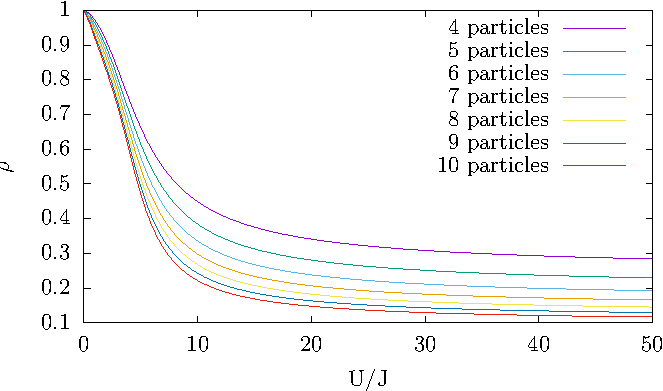
\includegraphics[width=\textwidth]{Figures/Condfrac_4to10.pdf}
        \caption{\textit{Condensate fraction calculated using the DMRG algorithm.}}
        \label{fig:Condfrac_4to10}
    \end{subfigure}
    ~
    \begin{subfigure}[t]{0.49\textwidth}
        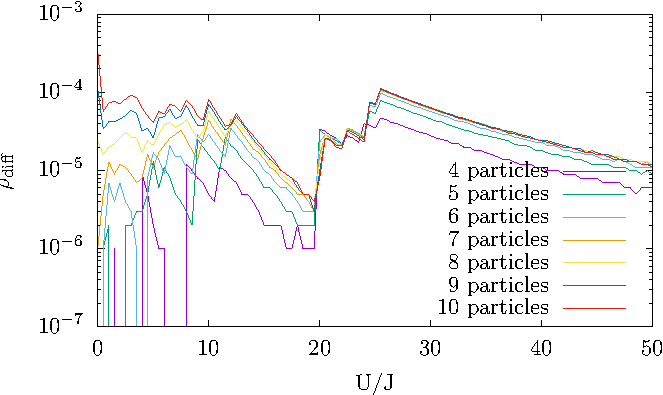
\includegraphics[width=\textwidth]{Figures/Confrac_exactvsMPS.pdf}
        \caption{\textit{Absolute difference between the condensate fraction calculated using DMRG and exact diagonalisation.}}
        \label{fig:Condfrac_exactvsMPS}
    \end{subfigure}    
\end{figure}
Figure \ref{fig:Condfrac_4to10} shows the condensate fraction for various $U/J$ calculated using the DMRG algorithm. In the limit $U/J = 0$, the condensate fraction is unit, confirming the system is indeed in the Superfluid phase. The condensate fraction never reaches zero, as $U/J$ increases, since this is only achieved in the thermodynamic limit. However, the condensate fraction does decrease with increasing particle number, as would be expected.\\
In figure \ref{fig:Condfrac_exactvsMPS} the results of the DMRG calculation is compared to exact diagonalisation. For small systems the two approaches obtain very similar results.\\
Attempting to use exact diagonalisation for large systems is futile, due to the exponential scaling of the Hilbert space \cite{Vidal2003}. However, this is not an issue using matrix product states, as the formalism only considers a tiny corner of the Hilbert space by following an area law. 
\begin{figure}[h!]
	\centering
	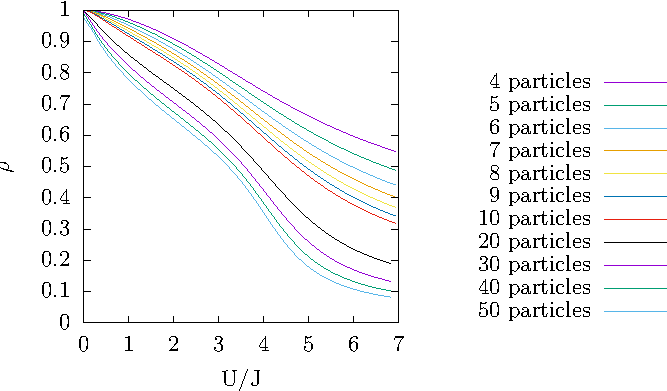
\includegraphics[width=0.9\textwidth]{Figures/Condfrac_4to50.pdf}
	\caption{\textit{Condensate fraction calculated using the DMRG algorithm with 20 sweeps.}}
	\label{fig:Condfrac_4to50}
\end{figure}
Figure \ref{fig:Condfrac_4to50} shows the results of the DMRG calculations for up to 50 particles. The condensate fraction behaves as expected in the $U/J \gg 1$ limit, as it tends towards zero for larger particle numbers. Note, in the Superfluid limit the condensate fraction does not quite reach 1. This is due to difficulty of describing long-range correlations when using matrix product states. An extensive explanation of this is given in Section \ref{sec:correlationFunctions}.
This is not an issue for smaller systems, as the correlation length is limited by the system size, due to boundary effects having an influence on a much larger part of the system. \\
Some measures can be taken to minimize errors, when using the DMRG algorithm. Accurately describing long range correlations requires multiple sweeps, as the algorithm has to iteratively approximate an almost constant function with a series of exponentials. Figure \ref{fig:sweepdependence} displays the condensate fraction in the Superfluid limit as a function of number of sweeps. Clearly, performing more sweeps yields a better result.
\begin{figure}[h!]
    \centering
    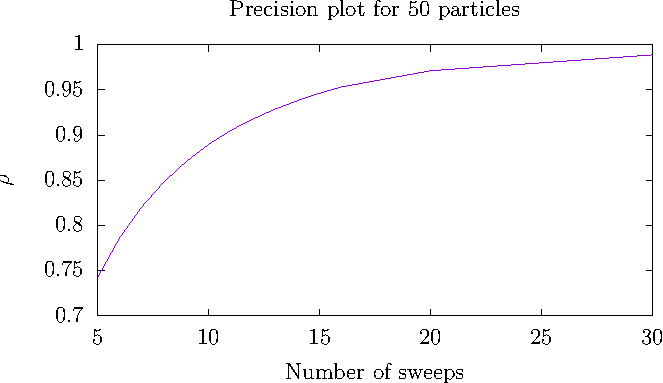
\includegraphics[width=0.8\textwidth]{Figures/condFracSweeps.pdf}
    \caption{\textit{Condensate fraction as a function of number of sweeps of the DMRG algorithm in the Superfluid limit. A max bond dimension of 250 was used.}}
    \label{fig:sweepdependence}
\end{figure}
Furthermore, increasing the maximal bond dimension, $D$, results in a more accurate long-range representation of correlations. Thus, calculating correlation functions for various values of $D$ is a great way of estimating the convergence of the correlations for a given length scale \cite{schollwock}.\\

In \cite{Kuhner2000} the critical point of phase transition between the Superfluid and Mott-Insulator is determined as $\left( \frac{U}{J} \right)_{crit} = 3.37$. The result is achieved through examining the correlations of the systems. While correlations in Mott-Insulators decay exponentially, Superfluids have a decay of correlations following the power-law given in eq. \eqref{sec:correlationFunctions}. As a result, the interface between the two phases, which can be seen in figure \ref{fig:SFMOTT}, has correlations following a power law determined by the Luttinger liquid parameter. The critical point, which is located at the tip of the Mott-lobes, is computed by determining the point, at which the Luttinger liquid parameter is $K =  \frac{1}{2}$. CITE\\
Examining figure \ref{fig:Condfrac_4to50}, one notices a hump on the graph in the vicinity of this critical ratio, but no clear indication of a phase transition is present. In the thermodynamic limit, one would expect the condensate fraction to drop to zero, as the critical ratio is reached (as observed in 2D by \cite{Spielman2008}). However, at 50 particles the condensate fraction is only around $ f_c = 0.5$. One could extrapolate data from computations using different particle numbers in order to determine the location of the critical point. However, this would require computations using larger systems in order to minimize the boundary effects.